\documentclass[crop,class=article]{standalone}
%----------------------------Preamble-------------------------------%
\usepackage{pgfplots, tikz}             % Drawing/graphing tools.
\usetikzlibrary{arrows.meta}            % Latex and Stealth arrows.
\pgfplotsset{compat=1.9}                % Version of pgfplots.
%--------------------------Main Document----------------------------%
\begin{document}
    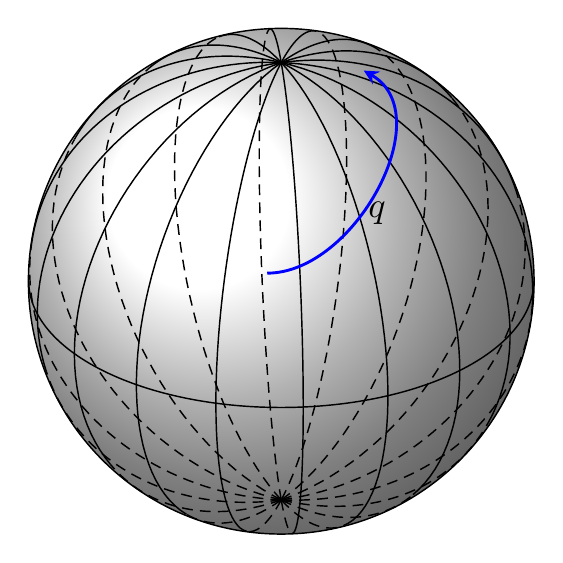
\begin{tikzpicture}[scale=1.3]
        \begin{axis}[%
            axis equal,
            width=14cm,
            height=14cm,
            hide axis,
            enlargelimits=0.3,
            view/h=45,
            view/v=30,
            scale uniformly strategy=units only,
            colormap={bluewhite}{%
                color=(blue) color=(white)%
            }
        ]
            \coordinate (X) at (axis cs: 1,0,0);
            \coordinate (-X) at (axis cs: -1,0,0);
            \coordinate (Y) at (axis cs: 0,1,0);
            \coordinate (-Y) at (axis cs: 0,-1,0);
            \coordinate (Z) at (axis cs: 0,0,1);
            \coordinate (-Z) at (axis cs: 0,0,-1);
            \draw[ball color=white] (axis cs: 0,0,0) circle (2.47cm);
            \coordinate (X) at (axis cs: 1,0,0);
            \draw (X) arc (0:45:100) (X) arc (0:-135:100);
            \foreach\a in {0,20,...,340}{%
                \pgfmathsetmacro{\Bound}{-60*cos(\a+45)}
                \addplot3[%
                    domain=\Bound:90,
                    samples=45,
                    samples y=0%
                ]   ({cos(\a)*cos(x)},{sin(\a)*cos(x)},{sin(x)});
                \addplot3[%
                    domain=-90:\Bound,
                    samples=45,
                    samples y=0,
                    densely dashed%
                ]   ({cos(\a)*cos(x)},{sin(\a)*cos(x)},{sin(x)});
            }
            \draw[draw=blue, >={stealth[blue]} ,->,thick]
                (3.2cm,3.5cm,3.5cm) to [in=330, out=0]
                node [below] {$q$} (2.0cm,6.6cm,5cm);
        \end{axis}
    \end{tikzpicture}
\end{document}